\documentclass[a4paper,10pt]{article}

\usepackage[utf8]{inputenc}
\usepackage[english,spanish]{babel}
\usepackage{graphicx}
\usepackage{url}
\usepackage[pageanchor=false,colorlinks,linkcolor=black,anchorcolor=black,
citecolor=black]{hyperref}
\usepackage{float}
\restylefloat{table}

\title{Servicio de domótica\\ Grupo 3}
\author{Omar \'Alvarez Mures \\
	Noelia Luaces Fern\'andez \\
	Adri\'an Mor\'an Garc\'ia \\
	Alfonso Nishikawa Mu\~numer \\
	David Torres Andreu}
\date{}

\hypersetup{pdfinfo={
Title={Servicio de domótica},
Author={Omar \'Alvarez Mures,
	Noelia Luaces Fern\'andez,
	Adri\'an Mor\'an Garc\'ia,
	Alfonso Nishikawa Mu\~numer,
	David Torres Andreu},
Subject={},
Keywords={}
}}

\hypersetup{
    %bookmarks=true,         % show bookmarks bar?
    unicode=true,          % non-Latin characters in Acrobat’s bookmarks
    pdftoolbar=false,        % show Acrobat’s toolbar?
    pdfmenubar=true,        % show Acrobat’s menu?
    pdffitwindow=false,     % window fit to page when opened
    pdfstartview={FitH},    % fits the width of the page to the window
    pdftitle={Servicio de domótica},    % title
    pdfauthor={Omar \'Alvarez Mures, Noelia Luaces Fern\'andez, Adri\'an Mor\'an 
Garc\'ia, Alfonso Nishikawa Mu\~numer, David Torres Andreu},     % author
    pdfsubject={Arquitectura do Software},   % subject of the document
    pdfcreator={Kile 2.1.3},   % creator of the document
    pdfproducer={Kile 2.1.3}, % producer of the document
    pdfkeywords={software architecture} {erlang}, % list of keywords
    pdfnewwindow=true,      % links in new window
    colorlinks=true,       % false: boxed links; true: colored links
    linkcolor=black,          % color of internal links (change box color with linkbordercolor)
    citecolor=black,        % color of links to bibliography
    filecolor=black,      % color of file links
    urlcolor=black           % color of external links
}

\begin{document}

\maketitle

\newpage

\section{Descripción del trabajo}

\subsection{Descripción del entorno de negocio}
El proyecto consistirá en el desarrollo de un sistema que monitorice el 
estado de los diferentes sistemas domóticos que contiene una vivienda 
determinada dotándola de los principales servicios de gestión energética, 
seguridad y bienestar. El sistema monitorizará cada sensor de cada habitación, 
organizándose por zonas.

En el interior de la casa, controlaremos la climatización, iluminación, 
persianas y humo, y en la zona exterior de la vivienda (patio) controlaremos 
iluminación y tendremos un sensor de movimiento.

\subsection{Requisitos funcionales}
Un cliente se podrá conectar al servicio de monitorización para consultar el 
estado de los distintos sensores. Para ello el sistema se encargará de comprobar 
qué elementos están activos y cuáles no, permitiendo obtener los distintos 
valores de los sensores. El sistema debe permitir la agrupación de monitores 
según  criterios del usuario. 

\subsection{Requisitos no funcionales}
El sistema tratará de garantizar, en la medida de lo posible, la disponibilidad 
del servicio de lectura de sensores, siempre y cuando no sea un fallo propio del 
sensor.

El sistema debe poder escalar la cantidad de sensores a monitorizar garantizando 
el óptimo rendimiento del servicio.

Para garantizar el rendimiento, cuando los esclavos mueren, se crea un nuevo 
esclavo.

Asimismo, el sistema podrá soportar facilidad de prueba debido a sus capas, ya 
que permite la realización de las pruebas, teniendo sensores virtuales.

\newpage

\section{Objetivos concretos del trabajo}

\subsection{Arquitectura a aplicar}
La arquitectura a utilizar en el sistema será de tipo Maestro-Esclavo, donde 
habrá un maestro principal, encargado de interactuar con el cliente, que 
controlará una subcapa de maestros que organizarán a los esclavos por grupos.

El maestro principal podrá levantar a los maestros de la capa inferior que 
agrupan a los monitores de sensores, en el caso de que se encuentren caídos. Los 
maestros de la subcapa podrán levantar a los monitores de sensores que a su vez 
se encuentren caídos.

Los monitores de sensores aligerarán la carga de procesado a los maestros, 
haciendo un filtrado de los valores del sensor en caso de que haya una 
diferencia importante en los valores. Es decir, el esclavo (monitor de sensor) 
informará al maestro en el caso de que haya un salto importante en los valores 
de un sensor determinado.

\begin{figure}[h!]
  \centering
  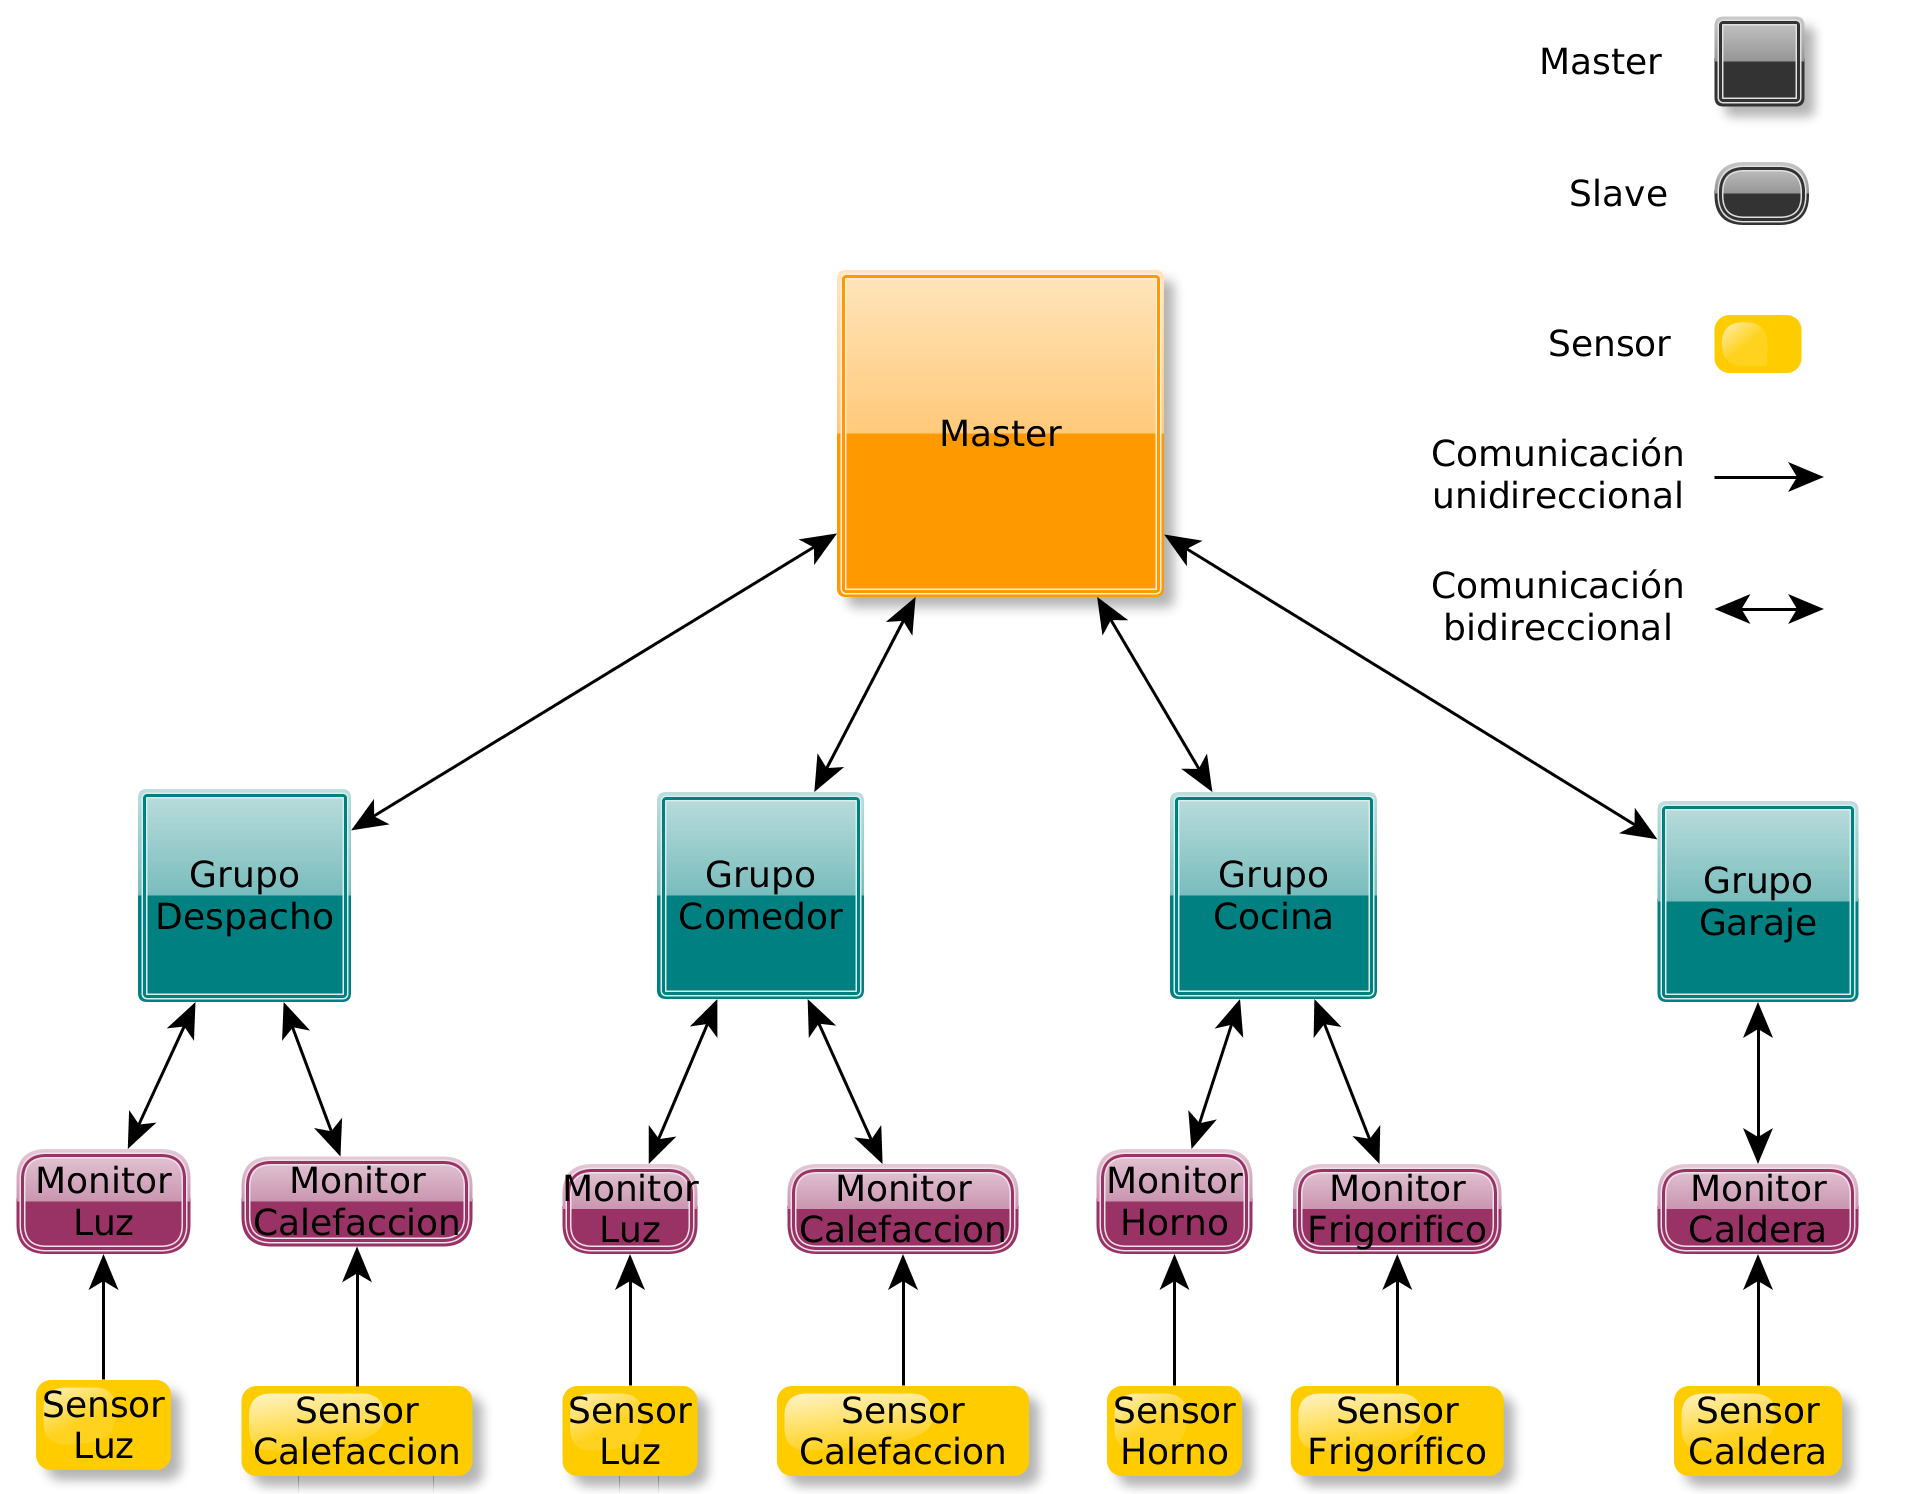
\includegraphics[width=\textwidth]{images/arch.png}
  \caption{Esquema de la arquitectura a implantar}
  \label{fig:arch}
\end{figure}

\subsection{Tácticas a aplicar}
\begin{enumerate}
  \item Tácticas de disponibilidad
  \begin{enumerate}
    \item Detección de errores
    \begin{description}
      \item [Ping] Se utilizará esta táctica entre los maestros y los grupos, 
para saber si es necesario levantarlos o no.
      \item [Heartbeat] Los monitores de sensores harán uso de esta táctica para 
informar de que están levantados, y a mayores proporcionar información 
adicional, como por ejemplo el cambio brusco de valores de los sensores.
      \item [Excepciones] Los componentes que se mueren lanzan excepciones y los 
componentes enlazados tratan dicha excepción y relanzan de nuevo los componentes 
que la han lanzado.
    \end{description}
    
    \item Recuperación de errores
    \begin{description}
      \item [Repuesto] Se incluye un componente equivalente en función de si 
falla o no.
    \end{description}
    
    \item Prevención de errores
    \begin{description}
      \item [Monitor de procesos] El master monitoriza el estado de los grupos y 
cada grupo monitoriza el estado de cada monitor de sensor.
    \end{description}
  \end{enumerate}
  
  \item Tácticas de flexibilidad al cambio
  \begin{enumerate}
    \item Localización de modificaciones
    \begin{description}
      \item [Coherencia semántica] Los servicios comunes tienen el mismo tipo de 
componentes, como por ejemplo los grupos o los monitores de sensores.
      \item [Anticipación de cambios esperables] Al aislar la lógica de la 
monitorización de sensores, su cambio no afecta a los grupos o al master, debido 
a que éstos sólo gestionan el uso de los monitores de sensores.
      \item [Generalización de cambios] Se utiliza en conjunto con la anterior 
táctica, debido a que no podemos anticiparnos a todos los cambios. Intentamos 
generalizar lo máximo posible para finalmente reducir el impacto de los mismos.
    \end{description}
    \item Prevención de efecto dominó
    \begin{description}
      \item [Ocultación de información] El maestro y los grupos delegan la 
lógica de los monitores de los sensores, esperando únicamente la respuesta; sin 
conocer el API concreto.
      \item [Uso de intermediarios] El cliente se comunicará con los monitores a 
través del master, y éste con los sensores a través de los monitores.
    \end{description}
    \item Postergación de la ligadura
    \begin{description}
      \item [Ligadura dinámica] Carga de código en caliente. Los módulos 
incluirán sentencias para actualizar a la última versión compilada del código.
    \end{description}
  \end{enumerate}
  
  \item Tácticas de rendimiento
  \begin{enumerate}
    \item Demanda de recursos
    \begin{description}
      \item [Gestión del ratio de eventos] Reducimos la frecuencia con la que se 
comprueba el valor de los sensores por los monitores de sensores sólo para 
aquellos casos cuyo umbral de variación sea significativo.
      \item [Control de frecuencia de muestreo] Se reduce la frecuencia de 
los eventos que le llegan a los grupos sin que éstos tengan control sobre su 
ratio de llegada.
      \item [Limitación del tiempo de ejecución] Si se realiza una petición y 
ésta supera un timeout determinado, la petición se deshecha.
      \item [Limitación de colas] En cada proceso se va a limitar el número de 
mensajes que pueden estar encolados.
    \end{description}
    \item Arbitraje de recursos
    \begin{description}
      \item [FIFO] Las peticiones del cliente al master serán atendidas en el 
orden de llegada, garantizando que todas serán satisfechas.
    \end{description}
  \end{enumerate}  
  
  \item Tácticas de facilidad de prueba
  \begin{enumerate}
    \item Gestión de entradas y salidas
    \begin{description}
      \item [Separación de interfaz/implementación] Los sensores serán 
simulados.
    \end{description}
  \end{enumerate}
  
  \item Tácticas de usabilidad
  \begin{enumerate}
    \item En tiempo de ejecución
    \begin{description}
      \item [Soporte a la iniciativa del sistema] El sistema enviará al 
usua\-rio información sobre el estado de los distintos grupos y monitores de sensores.
    \end{description}
  \end{enumerate}
\end{enumerate}
  
  
\newpage

\section{Plan inicial}

\begin{enumerate}
  \item Tareas para lograr los objetivos
  \begin{itemize}
    \item Estudio de los requisitos
    \item Análisis de las tácticas a utilizar
    \item Análisis y diseño de la arquitectura escogida
    \item Desarrollo del proceso cliente
    \item Desarrollo del proceso maestro
    \item Desarrollo del proceso grupo
    \item Desarrollo del proceso monitor de sensor
    \item Desarrollo del simulador del sensor
    \item Desarrollo de los casos de prueba
    \item Ejecución de las pruebas
    \item Elaboración de la documentación
  \end{itemize}

  \item Herramientas y tecnologías a utilizar
  \begin{itemize}
    \item Lenguaje de programación Erlang
    \item Eclipse
    \item EUnit
    \item EDoc
    \item Cover
    \item LaTeX
  \end{itemize}

  \item Estimación de esfuerzo de cada tarea
  \begin{table}[H]
    \centering
    \begin{tabular}{l r}
      Estudio de los requisitos & 8h \\
      Análisis de las tácticas a utilizar & 8h \\
      Análisis y diseño de la arquitectura a implantar & 9h \\
      Desarrollo del proceso cliente & 20h \\
      Desarrollo del proceso maestro & 20h \\
      Desarrollo del proceso grupo & 20h \\
      Desarrollo del proceso monitor de sensor & 20h \\
      Desarrollo del simulador del sensor & 20h \\
      Desarrollo de los casos de prueba & 8h \\
      Ejecución de las pruebas & 8h \\
      Elaboración de la documentación & 16h
    \end{tabular}
  \end{table}


  \item Lista de posibles riesgos durante el desarrollo
  \begin{itemize}
    \item Tareas subestimadas para el equipo actual por una falta de dominio en el lenguaje.
    \item Dentro de las tácticas escogidas, que haya tácticas que anulen parcialmente o resten beneficios a otras.
  \end{itemize}

\end{enumerate}

\end{document}
